\begin{figure}[H]
    \centering
    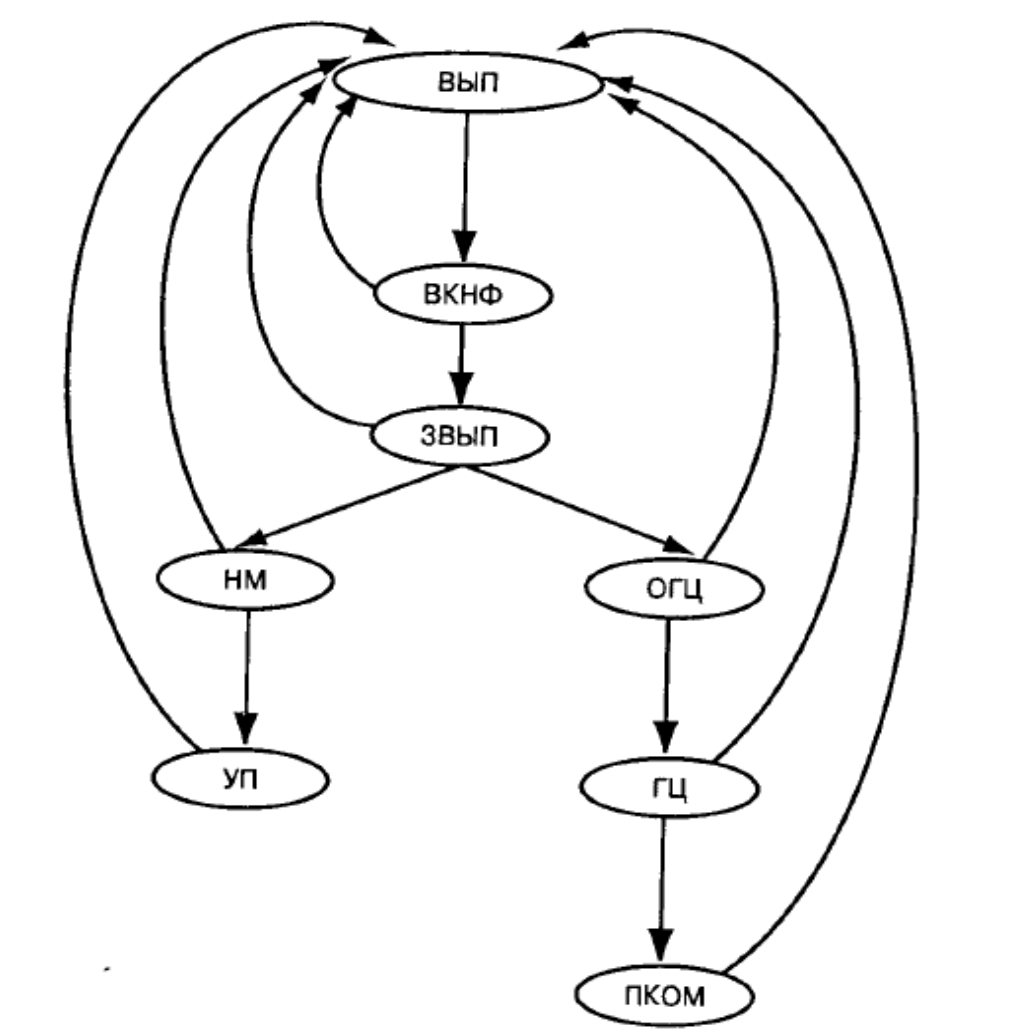
\includegraphics[height = 12cm]{images/np.png}
    \caption{Схема сведений $\mathscr{NP-}$полных проблем}
\end{figure}

\subsection*{Форма описания $\mathscr{NP}-$полной проблемы:}
\begin{enumerate}
    \item Название проблемы и ее аббревиатура
    \item Вход проблема: что и каким образом представляют данные
    \item Искомый выход: при каких условиях выходом будет <<да>>
    \item Известная проблема, сведение которой к данной проблеме доказывает $\mathscr{NP}-$полноту последней
\end{enumerate}

\subsection*{Проблемы выполнимости (ВЫП)}
\textbf{Формулы алгебры высказываний строятся из следующих элементов:}

1. Пропозициональные переменные, принимающие значения 1 (истина) или 0 (ложь)

2. Бинарные операторы $\land,\lor$, обозначающие логические связки И, ИЛИ двух формул

3. Унарный оператор $\lnot$, который обозначает логическое отрицание

4. Скобки для группирования операторов и операндов, если необходимо изменить порядок старшинства (приоритетов) операторов, принятый по умолчанию $(\lnot,\land,\lor)$

\textbf{Представление экземпляров ВЫП}

Используется следующий код:

1. Символы $\land,\lor,\lnot$, и скобки $(,)$ представляют самих себя

2. Переменная $X_i$ представляется символом $X$ с дописанной к нему последовательностью нулей и единиц -- двоичной записью числа $i$

Таким образом, алфавит $A$ проблемы"=языка ВЫП содержит всего 8 символов. Все экземпляры ВЫП являются цепочками символов -- словами в этом фиксированном конечном алфавите.

\textbf{Проблема выполнимости (ВЫП)}

\textbf{Вход:} слова $w$ в алфавите $A$, кодирующие экземпляры формулы алгебры высказываний $\Phi$ -- экземпляры ВЫП.

\textbf{Выход:} значение 1 -- ответ <<да>> -- тогда и только тогда, когда закодированная формула алгебры высказываний $\Phi$ выполнима.

\underline{Проблемы выполнимости (ВЫП)} формул алгебры высказываний состоит в следующем: необходимо выяснить, выполнима ли данная формула алгебры высказываний $\Phi$?

\underline{Теорема Кука.} Проблема ВЫП $\mathscr{NP}-$полна.

\subsection*{Проблемы выполнимости (ВКНФ)}
\begin{itemize}
    \item Выяснить, выполнима ли данная формула алгебры высказываний $\Phi$ в форме КНФ?
\end{itemize}

\textbf{Вход проблемы ВКНФ:}

слова $w$ в алфавите $A$, кодирующие формулы алгебры высказываний $\Phi$ в форме КНФ -- экземпляры ВКНФ.

\textbf{Искомый выход:}

значение 1 -- ответ <<да>> -- тогда и только тогда, когда закодированная формула алгебры высказываний $\Phi$ выполнима.

\textbf{Известная $\mathscr{NP-}$полная проблема}, которая сводится к ВКНФ -- проблема ВЫП.

\begin{theorem}
    Для любой формулы алгебры логики $\Phi$ за полиномиальное время можно построить такую формулы алгебры логики $\Phi'$ в форме КНФ, что выполняются условия:
    \begin{enumerate}
        \item Форумала $\Phi$ выполнима в том и только том случае, если выполнима КНФ $\Phi'$
        \item Длина формулы $\Phi'$ линейно зависит от количества символов в формуле $\Phi$
    \end{enumerate}
\end{theorem}

\textit{Доказательство:} индукцией по числу символов операций в формуле $\Phi$ проносим отрицания к переменным и затем индукцией по длине формулы получаем формулу $\Phi'$ в форме КНФ.

\begin{theorem}
    Проблемы ВЫП полиномиально сводится к проблеме ВКНФ.
\end{theorem}

\begin{corollary}
    Проблема ВКНФ $\mathscr{NP-}$полная.
\end{corollary}

\subsection*{Ограниченная проблемы выполнимости (3-ВЫП)}

\begin{itemize}
    \item Выяснить, выполнима ли данная формула алгебры высказываний $\Phi$ в форме КНФ с дизъюнктами из 3 литер?
\end{itemize}

\textbf{Вход проблемы 3-ВЫП:}

слова $w$ в алфавите $A$, кодирующие формулы алгебры высказываний $\Phi$ в форме КНФ с дизъюнктами из 3 литер -- экземпляры ВКНФ.

\textbf{Искомый выход:}

значение 1 -- ответ <<да>> -- тогда и только тогда, когда закодированная формула $\Phi$ выполнима.

\textbf{Известная $\mathscr{NP-}$полная проблема,} которая сводится к 3-ВЫП -- проблема ВКНФ.

\begin{theorem}
    Для любой формулы алгебры высказываний $\Phi$ в форме КНФ за полиномиальное время можно построить такую формулу алгебры высказываний $\Phi'$ в форме КНФ с дизъюнктами из 3 литер, что выполняются условия:
    \begin{enumerate}
        \item Формула $\Phi$ выполнима в том и только том случае, если выполнима КНФ $\Phi'$
        \item Длина формулы $\Phi'$ линейно зависит от количества символов в формуле $\Phi$
    \end{enumerate}
\end{theorem}
\textit{Доказательство:} индукцией по числу символов операций в дизъюнктах формулы $\Phi$ получаем формулу $\Phi'$ в форме КНФ с дизъюнктами из 3 литер.

\begin{theorem}
    Проблема ВКНФ полиномиально сводится к проблеме 3-ВЫП.
\end{theorem}

\begin{corollary}
    Проблема 3-ВЫП $\mathscr{NP-}$полна.
\end{corollary}

\subsection*{Проблема независимого множества (НМ)}
\begin{figure}[H]
    \centering
    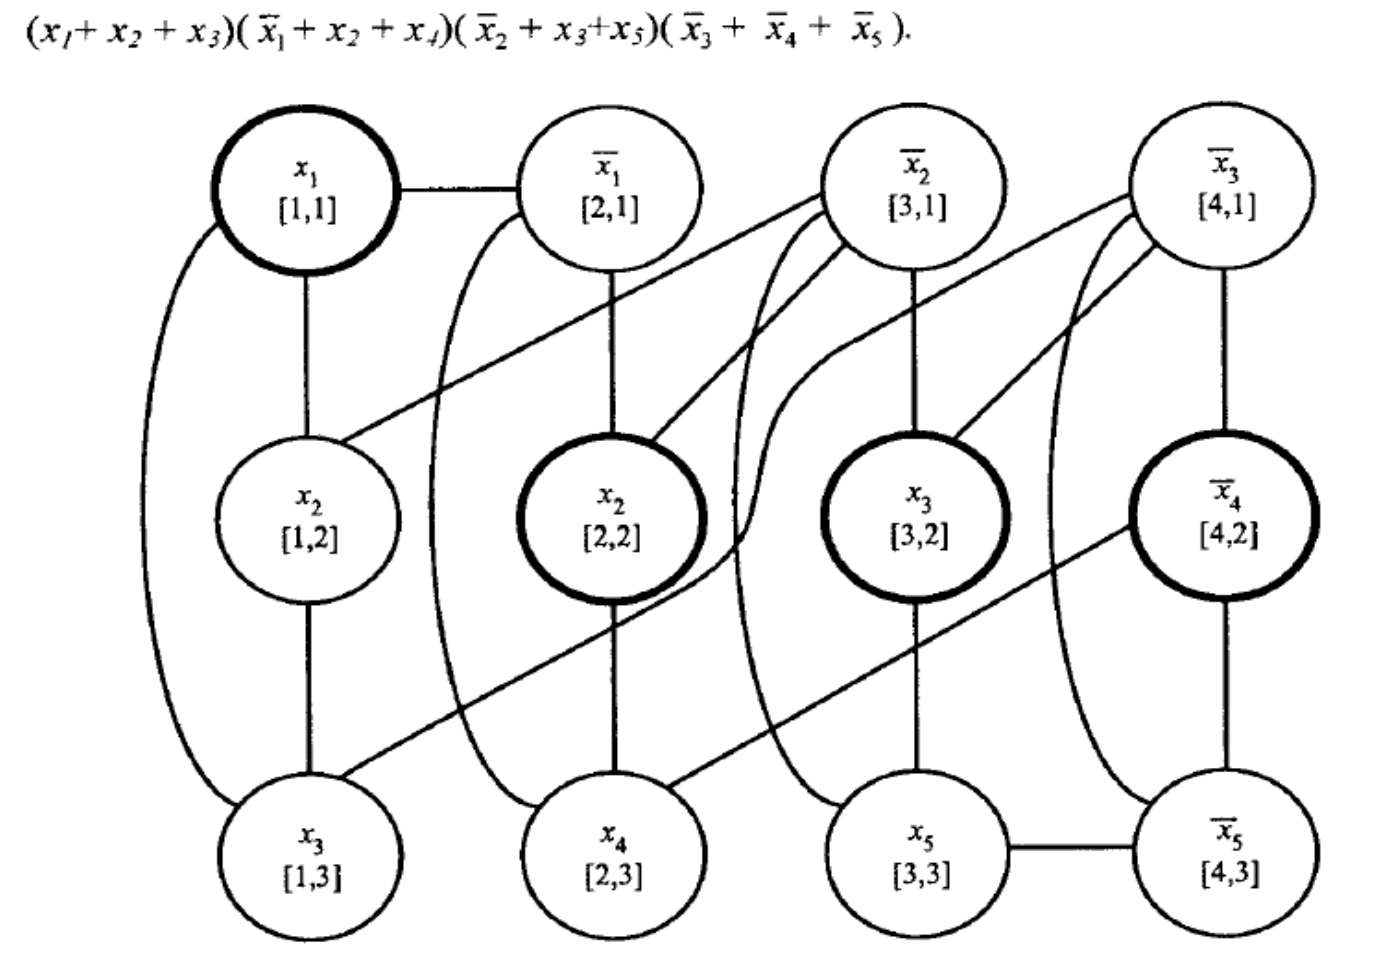
\includegraphics[height = 10cm]{images/independent.png}
    \caption{Построение независимого множества по выполнимой булевой формуле, находящейся в 3-КНФ}
\end{figure}

\textbf{Вход:} граф $G=(V, E)$ и нижняя граница $k$, удовлетворяющая условию $1\leq q \leq |V|$.

\textbf{Выход:} ответ <<да>> тогда и только тогда, когда $G$ имеет независимое множество из $k$ вершин.

\textbf{Проблема, сводящаяся к данной:} Проблема 3-ВЫП.

\begin{corollary}
    Проблема независимого множества $\mathscr{NP-}$полна.
\end{corollary}

\subsection*{Проблема вершинного покрытия (ВП)}
\textbf{Вход:} граф $G=(V,E)$ и нижняя граница $k$, удовлетворяющая условию $0\leq k\leq |V|-1$.

\textbf{Выход:} ответ <<да>> тогда и только тогда, когда $G$ имеет вершинное покрытие из $k$ или менее числа вершин.

\textbf{Проблема, сводящаяся к данной:} Проблема НМ.

\begin{corollary}
    Проблема ВП $\mathscr{NP-}$полна.
\end{corollary}

\subsection*{Проблема ориентированного гамильтонова цикла (ОГЦ)}
\textbf{Вход:} ориентированный граф $G$.

\textbf{Выход:} ответ <<да>> тогда и только тогда, когда $G$ имеет ориентированный гамильтонов цикл.

\textbf{Проблема, сводящаяся к данной:} Проблема 3-ВЫП.

\begin{corollary}
    Проблема ОГЦ $\mathscr{NP-}$полна.

\subsection*{Проблема гамильтонова цикла (ГЦ)}
\textbf{Вход:} неориентированный граф $G$.

\textbf{Выход:} ответ <<да>> тогда и только тогда, когда $G$ имеет гамильтонов цикл.

\textbf{Проблема, сводящаяся к данной:} Проблема ОГЦ.

\begin{corollary}
    Проблема ГЦ $\mathscr{NP-}$полна.

\subsection*{Проблема коммивояжера (ПКОМ)}
\textbf{Вход:} взвешенный граф $G$ и предельное значение $k$.

\textbf{Выход:} ответ <<да>> тогда и только тогда, когда $G$ имеет гамильтонов цикл веса не превышающего $k$.

\textbf{Проблема, сводящаяся к данной:} Проблема ГЦ.

\begin{corollary}
    Проблема ПКОМ $\mathscr{NP-}$полна.

\subsection*{Задача целочисленного программирования (ЗЦП)}
\textbf{Вход:} система линейных ограничений, целевая функция и предельное значение $k$.

\textbf{Выход:} ответ <<да>> тогда и только тогда, когда функция имеет превышающее $k$ значение для допустимых переменных.

\textbf{Проблема, сводящаяся к данной:} Проблема 3-ВЫП.

\begin{corollary}
    Проблема ЗГЦ $\mathscr{NP-}$полна.